\documentclass[12pt,a4paper]{article}
\usepackage[utf8]{inputenc}
\usepackage{listings}
\usepackage{graphicx}
\usepackage{color}
\usepackage{xcolor}
\usepackage{caption}
\usepackage{subcaption}
\usepackage{hyperref}
\usepackage{tikz}
\usetikzlibrary{arrows,automata}

\definecolor{mygreen}{rgb}{0,0.6,0}
\definecolor{mygray}{rgb}{0.5,0.5,0.5}
\definecolor{mymauve}{rgb}{0.58,0,0.82}

\lstset{ %
  backgroundcolor=\color{blue!5},   % choose the background color; you must add \usepackage{color} or \usepackage{xcolor}
  basicstyle=\footnotesize,        % the size of the fonts that are used for the code
  breakatwhitespace=false,         % sets if automatic breaks should only happen at whitespace
  breaklines=true,                 % sets automatic line breaking
  captionpos=b,                    % sets the caption-position to bottom
  commentstyle=\color{mygreen},    % comment style
  deletekeywords={...},            % if you want to delete keywords from the given language
  escapeinside={\%*}{*)},          % if you want to add LaTeX within your code
  extendedchars=true,              % lets you use non-ASCII characters; for 8-bits encodings only, does not work with UTF-8
  frame=single,                    % adds a frame around the code
  keepspaces=true,                 % keeps spaces in text, useful for keeping indentation of code (possibly needs columns=flexible)
  keywordstyle=\color{blue},       % keyword style
  language=java,                 % the language of the code
  otherkeywords={},            % if you want to add more keywords to the set
  numbers=left,                    % where to put the line-numbers; possible values are (none, left, right)
  numbersep=5pt,                   % how far the line-numbers are from the code
  numberstyle=\tiny\color{mygray}, % the style that is used for the line-numbers
  rulecolor=\color{black},         % if not set, the frame-color may be changed on line-breaks within not-black text (e.g. comments (green here))
  showspaces=false,                % show spaces everywhere adding particular underscores; it overrides 'showstringspaces'
  showstringspaces=false,          % underline spaces within strings only
  showtabs=false,                  % show tabs within strings adding particular underscores
  stepnumber=2,                    % the step between two line-numbers. If it's 1, each line will be numbered
  stringstyle=\color{mymauve},     % string literal style
  tabsize=2,                       % sets default tabsize to 2 spaces
  title=\lstname                   % show the filename of files included with \lstinputlisting; also try caption instead of title
}


\lstset{basicstyle=\footnotesize\ttfamily,breaklines=true}
\lstset{frame=single}

\author{Lingyan Zhou}
\title{Week 3}
\begin{document}
\maketitle
\tableofcontents
\newpage

\section{Reflection}
My program acheives all the goals in the specification. I tested it on some interesting patterns found on the Internet, 
and my program behaved as expected.

The primary difficaulty was debugging. Initially, I cannot visualized the intermediate steps. I finnaly changed the file format
to png, with the help from the ImageReadWrite java class borrowed from CSC508. I can visualize the universe and thus
can find bugs more easily. And with the help from my C++ image processing code in CSC508, implementing border extrapolation
and simulation of the universe was not hard. What's hard is to find an interesting rule. I tried to simply change its 
born/stay-alive rules, say, to B234S234, but most of the time I got a totally random or totally dead universe in the end. However,
I did find an interesting rule.
\section{Interesting Rules}
I think an interesting rules makes the final state of the universe interesting. And an interesting universe should display some
repetitive patterns. For example, using the original rule set, the universe will not end up in a totally chaotic or empty state.
There are patterns like spaceships, sliders, or still lifes. In the universe produced by my ruleset (see Figure \ref{fig:r2out}), the whole universe is a stable pattern. 
\section{Testing My Code}
I tested my code by observing the output. I prepared some input data like spaceships, oscillators and still lifes. These patterns are predictable. I put some of the patterns on the edges so that I can test the border extrapolation functions. Then I run my program step by step and observe their outcomes. I also wrote the intermediate results to files. But the most used method was to create a simple pattern by clicking on the interface and press the "Step" button to see the result. For example, Figure \ref{fig:testing} shows a simple test case and its expected result.
\begin{figure}[h!]
        \centering
        \begin{subfigure}[b]{0.5\textwidth}
                \includegraphics[width=\textwidth]{../test/test1}
                \caption{Test input}
        \end{subfigure}%
        ~ %add desired spacing between images, e. g. ~, \quad, \qquad, \hfill etc.
          %(or a blank line to force the subfigure onto a new line)
        \begin{subfigure}[b]{0.5\textwidth}
                \includegraphics[width=\textwidth]{../test/test1-step2}
                \caption{Expected output after 2 steps}
                \label{fig:r2out}
        \end{subfigure}
        \caption{\label{fig:testing}Testing}
\end{figure}
\section{My Rule of the Universe}
Let me explain the rule I create for the universe. Besides alive and dead state, I added three more states. One is growing, one is dying and the other don't-care. Dont'-care state is used for borders and walls. A born and stay-alive condition is a predicate on the number of neighboring alive cells. In my current implementation, the one which produced Figure \ref{fig:r2out}, the born condition is that the 8-connected neighbors have 2 or 3 alive cells. and the stay-alive condition is that the 8-connected neighbors have 2, 3 or 4 alive cells.
The rule set has 7 rules:
\begin{enumerate}
\item If any born condition is met, a dead cell becomes alive.
\item If any born condition is met, a growing cell becomes alive.
\item If none born condition is met, a growing cell becomes dying.
\item If none stay-alive condition is met, an alive becomes dying.
\item If any stay-alive condition is met, an alive stays alive.
\item If any stay-alive condition is met, a dying cell becomes growing.
\item Otherwise, it will be dead.
\end{enumerate}
The ruleset is illustrated in Figure \ref{fig:statemachine}.
\begin{figure}[h!]
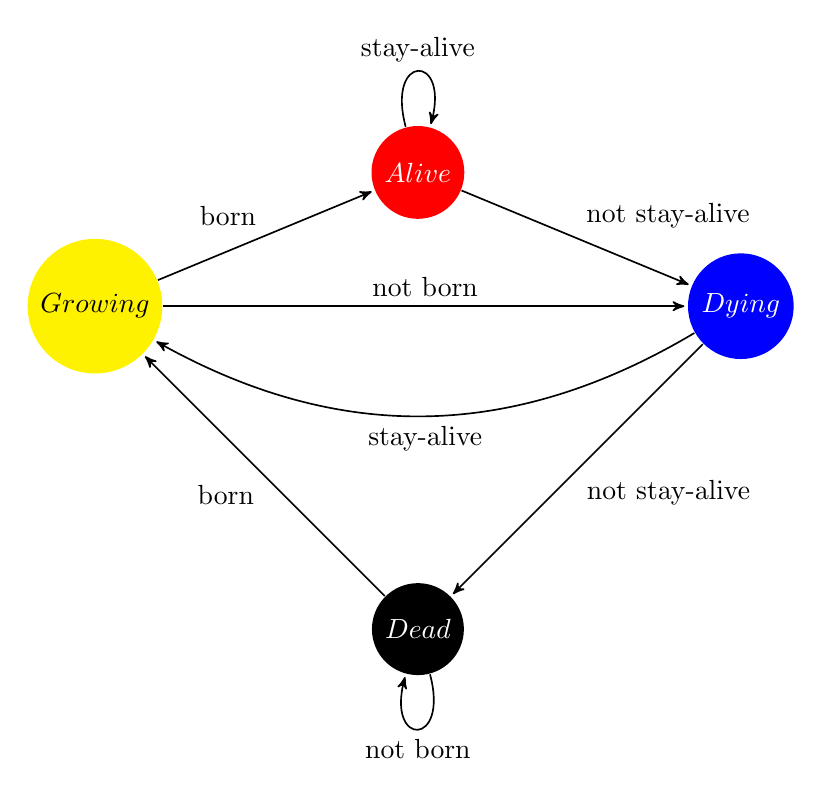
\begin{tikzpicture}[->,>=stealth',shorten >=1pt,auto,node distance=5.8cm,
                    semithick]
  \tikzstyle{every state}=[fill=red,draw=none,text=white]

  \node[state] (Dead)        [fill=black]            {$Dead$};
  \node[state]         (Growing) [above left of=Dead, fill=yellow, text=black] {$Growing$};
  \node[state]         (Alive) [above of=Dead, fill=red] {$Alive$};
  \node[state]         (Dying) [above right of=Dead, fill=blue] {$Dying$};

  \path (Dead) edge  [loop below]  node {not born} (Dead)
            edge              node {born} (Growing)
        (Growing) edge              node {born} (Alive)
            edge              node {not born} (Dying)
        (Alive) edge [loop above] node {stay-alive} (Alive)
            edge              node {not stay-alive} (Dying)
        (Dying) edge [bend left] node {stay-alive} (Growing)
            edge              node {not stay-alive} (Dead);
\end{tikzpicture}
\caption{\label{fig:statemachine}State transition of ruleset 2}
\end{figure}

For other information, you can refer to the javadoc in the /doc/ folder.


\newpage
\section{Screenshot}
\begin{figure}[h!]
        \centering
        \begin{subfigure}[b]{0.5\textwidth}
                \includegraphics[width=\textwidth]{r1out}
                \caption{Stablized universe on ruleset 1}
        \end{subfigure}%
        ~ %add desired spacing between images, e. g. ~, \quad, \qquad, \hfill etc.
          %(or a blank line to force the subfigure onto a new line)
        \begin{subfigure}[b]{0.5\textwidth}
                \includegraphics[width=\textwidth]{r2out}
                \caption{Stablized universe on ruleset 2}
                \label{fig:r2out}
        \end{subfigure}

        \caption{Stablized universe}
\end{figure}

\newpage
\section{Listings} 
\subsection{GameData.java}
\lstinputlisting[language=Java]{../src/GameData.java}
\subsection{DataPadding.java}
\lstinputlisting[language=Java]{../src/DataPadding.java}
\subsection{GameRule.java}
\lstinputlisting[language=Java]{../src/GameRule.java}
\subsection{GameRule1.java}
\lstinputlisting[language=Java]{../src/GameRule1.java}
\subsection{GameRule2.java}
\lstinputlisting[language=Java]{../src/GameRule2.java}
\subsection{ControlPanel.java}
\lstinputlisting[language=Java]{../src/ControlPanel.java}
\subsection{GraphicPanel.java}
\lstinputlisting[language=Java]{../src/GraphicPanel.java}
\subsection{ImageReadWrite.java}
\lstinputlisting[language=Java]{../src/ImageReadWrite.java}
\subsection{CellularAutomataFrame.java}
\lstinputlisting[language=Java]{../src/CellularAutomataFrame.java}


\end{document}
